%% 第三章

\chapter{基于受约束逆强化学习的对齐方法}
\chaptermark{基于受约束逆强化学习的对齐方法}

第一章已经指出，固定奖励模型会随着策略分布变化而逐渐失效。若在奖励-策略联合更新的逆强化学习框架下完全放开奖励模型更新，又会带来新的不稳定性：奖励函数变化过大时，策略优化会追逐不断漂移的奖励信号，导致奖励尺度膨胀或过优化。本章关注的问题是：在逆强化学习框架下，如何让奖励模型跟随策略分布持续更新，同时不让每一轮奖励更新幅度过大。本章先建立奖励学习与策略优化耦合的双层问题，再推导奖励函数诱导出的最优策略及原始目标。在此基础上构造固定旧策略的局部替代目标，证明其在展开点处与原始目标具有相同的一阶信息；给出带误差项的改进下界，刻画有限步更新后替代目标相对于原始目标的偏差；最后将这一约束思想转化为可计算的RMSD反馈机制，并给出完整训练流程。

从全文主题看，本章是“基于逆强化学习的大模型偏好对齐方法”的核心推导部分。这里的IRL不是一般意义上的模仿学习工具，而是用于刻画偏好目标的奖励反演过程：专家响应代表偏好行为，奖励函数表示待学习的偏好目标，策略优化则把该目标转化为语言模型的生成行为。PIRO的设计正是在这三个对象之间加入近端约束，使偏好奖励能够随策略更新而调整，同时保持跨轮变化可控。

\begin{figure}[H]
    \centering
    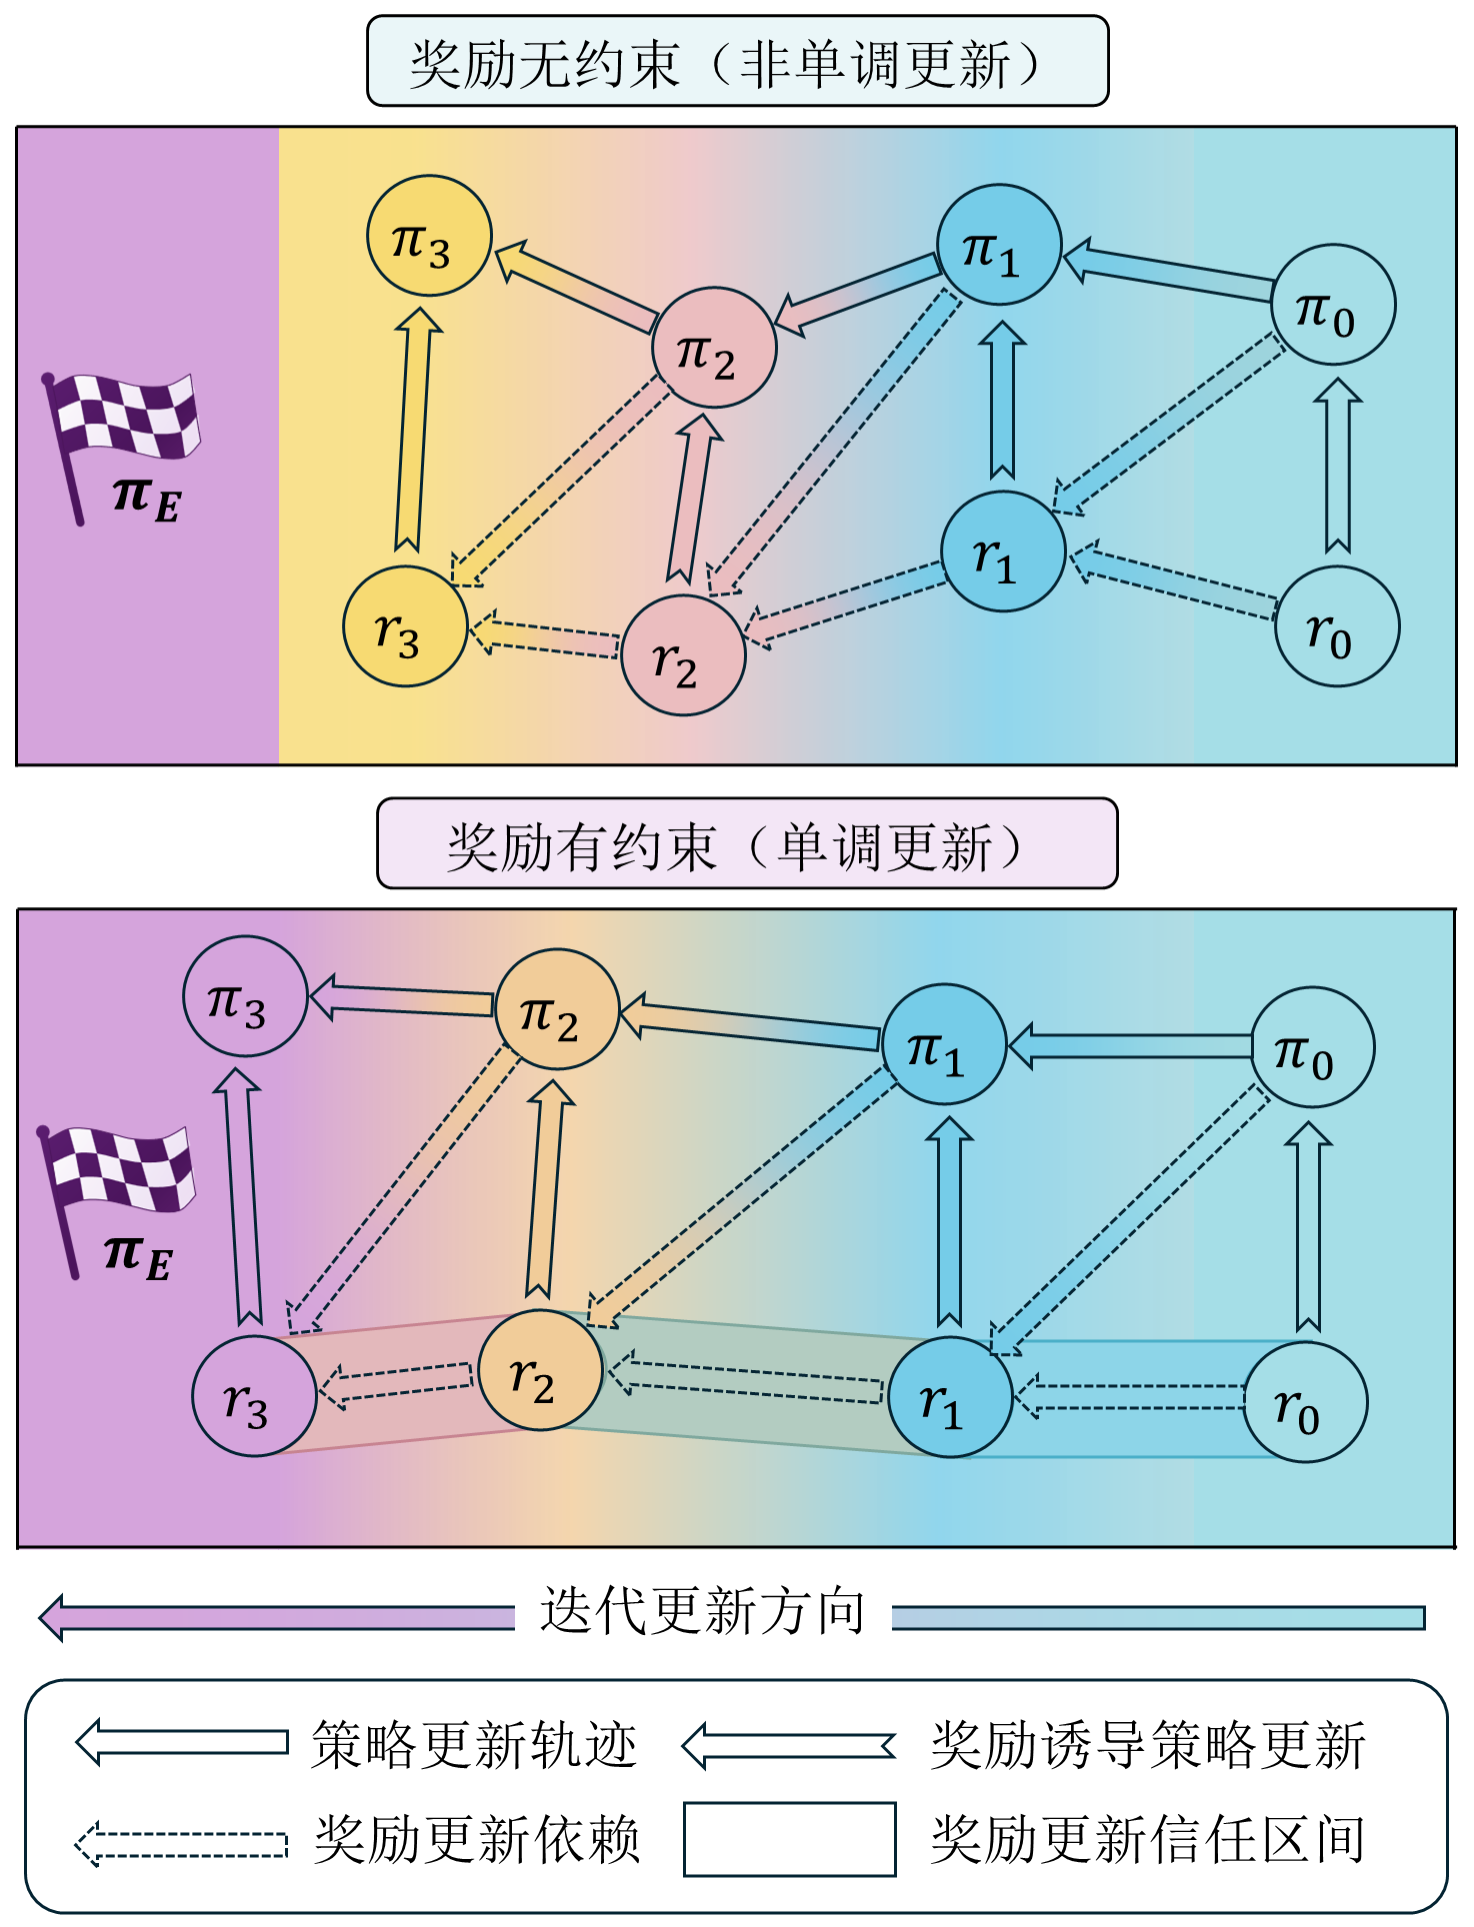
\includegraphics[width=0.60\textwidth]{figures/main.PNG}
    \caption{奖励约束对策略--奖励交替更新过程的影响示意}
    \label{fig:reward_constraint_overview}
\end{figure}

图~\ref{fig:reward_constraint_overview}给出了本章方法的直观动机。无约束奖励更新中，相邻轮次奖励函数会发生较大漂移，由奖励诱导出的策略更新方向也随之摆动，多轮迭代过程不一定稳定接近专家策略。受约束奖励更新将相邻奖励函数的变化限制在局部可信范围内，奖励诱导的策略更新轨迹相对平稳。后续各节对这一思想进行形式化：3.1节和3.2节建立奖励诱导策略及外层目标，3.3节证明固定旧策略得到的替代目标在展开点处具有一阶一致性，3.4节给出带误差项的改进下界，3.5节将理论中的奖励变化约束转化为可计算的RMSD反馈机制。

\section{问题建模}

\subsection{符号定义}

设 $\mathcal{X}$ 为提示空间，$\mathcal{Y}$ 为完整响应空间，$\rho$ 为提示分布。本文将大语言模型生成视为序列级单步决策过程：给定提示 $x$ 后，完整回答 $y$ 视为一次动作，因此动作价值函数 $Q(x,y)$ 可直接写成奖励 $r_\theta(x,y)$。$\pi_{\mathrm{E}}$ 表示专家响应分布，$\pi_{\mathrm{ref}}$ 表示参考策略，$\pi_\theta$ 表示由奖励函数 $r_\theta$ 诱导出的最优策略，$\beta>0$ 为KL正则系数。

\subsection{原始双层问题}

本文将策略-奖励学习问题形式化为如下双层优化问题：
\begin{equation}
\begin{aligned}
    \max_{\theta}\quad \ell(\theta)
    &:=\mathbb{E}_{x\sim\rho,\,y\sim\pi_{\mathrm{E}}(\cdot|x)}
    \left[\log \pi_\theta(y|x)\right],\\
    \mathrm{s.t.}\quad
    \pi_\theta
    &:=\arg\max_\pi\ \mathbb{E}_{x\sim\rho,\,y\sim\pi(\cdot|x)}
    \left[r_\theta(x,y)-\beta D_{\mathrm{KL}}\!\left(\pi(\cdot|x)\|\pi_{\mathrm{ref}}(\cdot|x)\right)\right].
    \label{eq:original_ch3}
\end{aligned}
\end{equation}
其中，外层目标用于学习奖励函数：通过调整奖励参数 $\theta$，让该奖励函数诱导出的策略 $\pi_\theta$ 倾向于生成专家响应；内层目标在给定奖励函数下优化策略，并通过KL正则限制新策略相对于参考策略的偏离。

该双层形式把大模型偏好对齐中的三个核心对象放在同一框架内：专家分布 $\pi_{\mathrm{E}}$ 提供偏好目标，奖励函数 $r_\theta$ 是该偏好目标的可学习表示，诱导策略 $\pi_\theta$ 则给出模型行为。后续推导围绕奖励函数展开，但最终目的始终是改善由奖励诱导出的策略分布，而不是单独提高奖励模型本身的数值。

\section{最优策略的闭式推导}

\subsection{内层问题的闭式解}

在序列级单步决策设定下，内层问题具有如下闭式解：
\begin{equation}
    \pi_\theta(y|x)=
    \frac{\pi_{\mathrm{ref}}(y|x)\exp\left(\frac{1}{\beta}r_\theta(x,y)\right)}
    {\sum_{\tilde{y}\in\mathcal{Y}}\pi_{\mathrm{ref}}(\tilde{y}|x)\exp\left(\frac{1}{\beta}r_\theta(x,\tilde{y})\right)}.
    \label{eq:pi_ch3}
\end{equation}
由式~\eqref{eq:pi_ch3}可见，奖励越高的响应在参考策略基础上获得更大的指数权重；$\beta$ 越大，KL约束越强，策略越接近参考模型。



\subsection{原始目标的等价表示}

为得到原始双层问题的显式外层目标，本节将内层最优策略的闭式解代入专家响应的对数似然目标，再改写为关于奖励函数及其诱导策略的等价形式。记式~\eqref{eq:pi_ch3}中的归一化项为：
\begin{equation}
    Z_\theta(x)=
    \sum_{\tilde{y}\in\mathcal{Y}}
    \pi_{\mathrm{ref}}(\tilde{y}|x)
    \exp\left(\frac{1}{\beta}r_\theta(x,\tilde{y})\right).
    \label{eq:z_ch3}
\end{equation}
由此，式~\eqref{eq:pi_ch3}可等价写为
\begin{equation}
    \beta\log\pi_\theta(y|x)
    =
    \beta\log\pi_{\mathrm{ref}}(y|x)
    +r_\theta(x,y)-\beta\log Z_\theta(x).
    \label{eq:log_pi_ch3}
\end{equation}
将式~\eqref{eq:log_pi_ch3}代入外层专家似然目标。$\pi_{\mathrm{ref}}$ 与 $\theta$ 无关，对应项可并入常数项，因此有
\begin{equation}
\begin{aligned}
    \beta\ell(\theta)
    &=
    \mathbb{E}_{x\sim\rho,\,y\sim\pi_{\mathrm{E}}(\cdot|x)}
    \left[r_\theta(x,y)-\beta\log Z_\theta(x)\right]
    +\mathrm{const}
\end{aligned}
\label{eq:ell_logz_ch3}
\end{equation}
同时，由式~\eqref{eq:pi_ch3}可得
\[
    r_\theta(x,y)-\beta\log\frac{\pi_\theta(y|x)}{\pi_{\mathrm{ref}}(y|x)}
    =\beta\log Z_\theta(x).
\]
右侧仅依赖于提示 $x$，对 $y\sim\pi_\theta(\cdot|x)$ 取期望得到
\[
    \beta\log Z_\theta(x)
    =
    \mathbb{E}_{y\sim\pi_\theta(\cdot|x)}
    \left[
    r_\theta(x,y)-\beta\log\frac{\pi_\theta(y|x)}{\pi_{\mathrm{ref}}(y|x)}
    \right].
\]
将上式代入式~\eqref{eq:ell_logz_ch3}后，可得到外层目标中依赖 $\theta$ 的部分。为让专家策略项与诱导策略项具有一致的KL正则形式，在不改变关于 $\theta$ 的优化问题的前提下，加入如下与 $\theta$ 无关的专家策略KL常数：
\[
    -\beta\mathbb{E}_{x\sim\rho}
    \left[D_{\mathrm{KL}}\!\left(\pi_{\mathrm{E}}(\cdot|x)\|\pi_{\mathrm{ref}}(\cdot|x)\right)\right].
\]
于是得到如下等价外层目标：
\begin{equation}
\begin{aligned}
    L(\theta)
    &=
    \mathbb{E}_{x\sim\rho,\,y\sim\pi_{\mathrm{E}}(\cdot|x)}
    \left[r_\theta(x,y)\right]
    -\beta\mathbb{E}_{x\sim\rho}
    \left[D_{\mathrm{KL}}\!\left(\pi_{\mathrm{E}}(\cdot|x)\|\pi_{\mathrm{ref}}(\cdot|x)\right)\right]\\
    &\quad-
    \mathbb{E}_{x\sim\rho,\,y\sim\pi_\theta(\cdot|x)}
    \left[r_\theta(x,y)-\beta D_{\mathrm{KL}}\!\left(\pi_\theta(\cdot|x)\|\pi_{\mathrm{ref}}(\cdot|x)\right)\right].
    \label{eq:l_from_ell_ch3}
\end{aligned}
\end{equation}
为便于后续表述，定义
\begin{equation}
\begin{aligned}
    J(\pi,r_\theta)
    &:={}
    \mathbb{E}_{x\sim\rho,\,y\sim\pi(\cdot|x)}
    \left[r_\theta(x,y)\right]
    -\beta\mathbb{E}_{x\sim\rho}
    \left[D_{\mathrm{KL}}\!\left(\pi(\cdot|x)\|\pi_{\mathrm{ref}}(\cdot|x)\right)\right].
\end{aligned}
\label{eq:j_ch3}
\end{equation}
由式~\eqref{eq:l_from_ell_ch3}和式~\eqref{eq:j_ch3}可得到外层目标的紧凑表示：
\begin{equation}
    L(\theta)=J(\pi_{\mathrm{E}},r_\theta)-J(\pi_\theta,r_\theta).
    \label{eq:l_objective_ch3}
\end{equation}
式~\eqref{eq:l_objective_ch3}是后续PIRO推导的起点。第一项刻画专家偏好响应在当前奖励下的正则化价值，第二项刻画该奖励诱导出的策略自身可达到的软最优值；二者之差反映奖励函数能否使专家行为在诱导策略分布中获得更高解释概率。由此，偏好对齐问题被具体化为受约束的奖励函数学习问题。

\section{替代目标的构造与一阶等价性}

\subsection{替代目标}

式~\eqref{eq:l_objective_ch3}给出了外层目标的紧凑表达，但它不适合直接作为每一轮奖励更新的训练目标。第二项中的 $\pi_\theta$ 由当前奖励函数 $r_\theta$ 诱导而来：当 $\theta$ 改变时，奖励函数改变，内层最优策略也随之改变。直接优化 $L(\theta)$ 会同时涉及奖励函数变化和诱导策略变化两个耦合因素，难以形成稳定的单步更新。

为降低上述耦合带来的优化难度，本节先在当前参数附近构造一个可优化的局部替代目标。在当前一轮奖励更新中固定上一轮策略 $\pi_{\mathrm{old}}=\pi_{\theta_{\mathrm{old}}}$，只更新奖励函数，构造如下替代目标：
\begin{equation}
    L_{\mathrm{old}}(\theta)=J(\pi_{\mathrm{E}},r_\theta)-J(\pi_{\mathrm{old}},r_\theta).
    \label{eq:surrogate_ch3}
\end{equation}
该替代目标的含义是：单轮奖励更新内不显式追踪 $\pi_\theta$ 随 $\theta$ 的变化，转而用固定的旧策略 $\pi_{\mathrm{old}}$ 替代原始目标中的诱导策略项。奖励更新的梯度由专家样本与旧策略样本之间的奖励差异估计得到。

\subsection{一阶等价性}

$L_{\mathrm{old}}$ 固定了原始目标中随 $\theta$ 改变的诱导策略项，因此不能视为 $L$ 的全局等价替代。本节只在展开点处验证其一阶一致性：当 $\pi_{\mathrm{old}}=\pi_{\theta_{\mathrm{old}}}$ 时，$L_{\mathrm{old}}$ 与 $L$ 在 $\theta_{\mathrm{old}}$ 处满足相同的函数值和梯度，即
\begin{equation}
    L(\theta_{\mathrm{old}})=L_{\mathrm{old}}(\theta_{\mathrm{old}}),
    \label{eq:first_order_value_ch3}
\end{equation}
\begin{equation}
    \nabla_\theta L(\theta)\big|_{\theta=\theta_{\mathrm{old}}}
    =\nabla_\theta L_{\mathrm{old}}(\theta)\big|_{\theta=\theta_{\mathrm{old}}}.
    \label{eq:first_order_grad_ch3}
\end{equation}
式~\eqref{eq:first_order_value_ch3}由 $\pi_{\mathrm{old}}=\pi_{\theta_{\mathrm{old}}}$ 直接得到；梯度一致性需要进一步计算。为保证推导成立，假设响应空间在给定最大生成长度下有限，奖励函数 $r_\theta(x,y)$ 关于 $\theta$ 可微，且 $\pi_{\mathrm{ref}}(y|x)>0$；专家响应分布与旧策略的支持均包含于参考策略支持内。

为计算原始目标的梯度，使用式~\eqref{eq:ell_logz_ch3}中显式依赖 $\theta$ 的形式。式~\eqref{eq:l_from_ell_ch3}中用于对称书写的专家策略KL项不依赖 $\theta$，其梯度为零，因此
\begin{equation}
\begin{aligned}
    \nabla_\theta L(\theta)
    &=\nabla_\theta\Bigg\{
    \mathbb{E}_{x\sim\rho,\,y\sim\pi_{\mathrm{E}}(\cdot|x)}
    \left[r_\theta(x,y)\right]
    -
    \beta\mathbb{E}_{x\sim\rho}\left[\log Z_\theta(x)\right]
    \Bigg\}.
\end{aligned}
    \label{eq:l_logz_ch3}
\end{equation}

记
\begin{equation*}
    A(\theta)=
    \mathbb{E}_{x\sim\rho,\,y\sim\pi_{\mathrm{E}}(\cdot|x)}
    \left[r_\theta(x,y)\right],\qquad
    B(\theta)=
    \mathbb{E}_{x\sim\rho}\left[\log Z_\theta(x)\right].
\end{equation*}
则
\begin{equation*}
    \nabla_\theta L(\theta)=\nabla_\theta A(\theta)-\beta\nabla_\theta B(\theta).
\end{equation*}
其中，第一项由奖励函数求导得到
\begin{equation*}
    \nabla_\theta A(\theta)
    =
    \mathbb{E}_{x\sim\rho,\,y\sim\pi_{\mathrm{E}}(\cdot|x)}
    \left[\nabla_\theta r_\theta(x,y)\right].
\end{equation*}
剩下的问题是计算第二项 $\nabla_\theta B(\theta)$。$B(\theta)=\mathbb{E}_{x\sim\rho}[\log Z_\theta(x)]$，因此只需先求固定提示 $x$ 下的 $\nabla_\theta\log Z_\theta(x)$。由式~\eqref{eq:z_ch3}可得
\begin{equation*}
\begin{aligned}
    \nabla_\theta \log Z_\theta(x)
    &=
    \frac{1}{Z_\theta(x)}
    \sum_{y\in\mathcal{Y}}\pi_{\mathrm{ref}}(y|x)
    \exp\left(\frac{1}{\beta}r_\theta(x,y)\right)
    \frac{1}{\beta}\nabla_\theta r_\theta(x,y)\\
    &=
    \frac{1}{\beta}
    \mathbb{E}_{y\sim\pi_\theta(\cdot|x)}
    \left[\nabla_\theta r_\theta(x,y)\right].
\end{aligned}
\end{equation*}
于是
\begin{equation*}
    \nabla_\theta B(\theta)
    =
    \frac{1}{\beta}
    \mathbb{E}_{x\sim\rho,\,y\sim\pi_\theta(\cdot|x)}
    \left[\nabla_\theta r_\theta(x,y)\right].
\end{equation*}
将 $\nabla_\theta A(\theta)$ 与 $\nabla_\theta B(\theta)$ 代入 $\nabla_\theta L(\theta)=\nabla_\theta A(\theta)-\beta\nabla_\theta B(\theta)$，得到原始目标的梯度：
\begin{equation*}
    \nabla_\theta L(\theta)
    =
    \mathbb{E}_{x\sim\rho,\,y\sim\pi_{\mathrm{E}}(\cdot|x)}
    \left[\nabla_\theta r_\theta(x,y)\right]
    -
    \mathbb{E}_{x\sim\rho,\,y\sim\pi_\theta(\cdot|x)}
    \left[\nabla_\theta r_\theta(x,y)\right].
\end{equation*}
另一方面，在替代目标 $L_{\mathrm{old}}(\theta)=J(\pi_{\mathrm{E}},r_\theta)-J(\pi_{\mathrm{old}},r_\theta)$ 中，$\pi_{\mathrm{E}}$、$\pi_{\mathrm{old}}$ 与 $\pi_{\mathrm{ref}}$ 都固定不随 $\theta$ 改变，KL项对 $\theta$ 的梯度为零，得到
\begin{equation*}
    \nabla_\theta L_{\mathrm{old}}(\theta)
    =
    \mathbb{E}_{x\sim\rho,\,y\sim\pi_{\mathrm{E}}(\cdot|x)}
    \left[\nabla_\theta r_\theta(x,y)\right]
    -
    \mathbb{E}_{x\sim\rho,\,y\sim\pi_{\mathrm{old}}(\cdot|x)}
    \left[\nabla_\theta r_\theta(x,y)\right].
\end{equation*}
将 $\theta=\theta_{\mathrm{old}}$ 代入上述两式即可得到式~\eqref{eq:first_order_grad_ch3}。替代目标在旧参数处与原始目标具有相同的函数值和一阶导数。该结论说明 $L_{\mathrm{old}}$ 可在展开点附近提供与 $L$ 一致的局部更新方向；但实际训练会从 $\theta_{\mathrm{old}}$ 移动到 $\theta_{\mathrm{new}}$，一旦离开展开点，替代目标仍会偏离原始目标。下一节对奖励函数的更新作进一步限制。

\section{改进下界定理}

上一节说明，固定旧策略后得到的替代目标 $L_{\mathrm{old}}$ 在 $\theta_{\mathrm{old}}$ 处与原始目标 $L$ 具有相同的一阶信息，可作为局部更新方向。但算法实际执行的是一次有限步更新，即从 $\theta_{\mathrm{old}}$ 移动到 $\theta_{\mathrm{new}}$。在新参数处，旧策略构造的替代目标未必仍然准确；如果替代目标对原始目标的高估过大，优化过程就只改进代理目标，而不能相应改进原始目标。

本节回答的问题是：参数从 $\theta_{\mathrm{old}}$ 更新到 $\theta_{\mathrm{new}}$ 后，替代目标相对于原始目标的高估误差能否被控制？式~\eqref{eq:lower_bound}给出了形式化回答。该式说明，若新旧奖励函数的逐点变化幅度 $\epsilon$ 较小，则 $L(\theta_{\mathrm{new}})$ 与 $L_{\mathrm{old}}(\theta_{\mathrm{new}})$ 之间的偏差受到 $C\epsilon$ 控制。3.3节给出展开点处的一阶一致性，本节给出有限步更新后的误差控制，二者共同构成后续受约束奖励更新方法的理论基础。

本节中，我们将证明式~\eqref{eq:lower_bound}。先定义奖励函数的最大逐点变化 $\epsilon$，将下界证明转化为控制差值 $L_{\mathrm{old}}(\theta_{\mathrm{new}})-L(\theta_{\mathrm{new}})$；再建立两个辅助界，分别控制新旧奖励诱导策略之间的全变差距离以及KL项中的对数策略比；最后将上述差值展开为奖励差异项与KL差异项，分别利用辅助界控制二者，得到式~\eqref{eq:lower_bound}。

\subsection{定理陈述}

定义相邻两轮奖励函数的最大逐点变化为
\begin{equation}
    \epsilon=
    \max_{x,y}\left|r_{\theta_{\mathrm{new}}}(x,y)-r_{\theta_{\mathrm{old}}}(x,y)\right|.
    \label{eq:epsilon_def}
\end{equation}
若 $|\mathcal{Y}|<\infty$，且对任意 $(x,y)$ 有 $|r_{\theta_{\mathrm{new}}}(x,y)|\le R$、$|r_{\theta_{\mathrm{old}}}(x,y)|\le R$，则有如下下界：
\begin{equation}
\begin{gathered}
    L(\theta_{\mathrm{new}})
    \ge
    L_{\mathrm{old}}(\theta_{\mathrm{new}})-C\epsilon,\\
    C=\frac{3R|\mathcal{Y}|}{\beta}.
    \label{eq:lower_bound}
\end{gathered}
\end{equation}
该定理说明，替代目标相对于原始目标的高估误差可由奖励函数变化幅度 $\epsilon$ 控制；当 $\epsilon$ 过大时，误差项 $C\epsilon$ 会抵消替代目标带来的改进。

\subsection{策略全变差距离引理}

先要控制新旧奖励函数诱导出的策略差异。令 $\pi_1=\pi_{\theta_{\mathrm{new}}}$、$\pi_2=\pi_{\theta_{\mathrm{old}}}$，本小节证明二者的全变差距离满足
\[
    D_{\mathrm{TV}}\left(\pi_1(\cdot|x),\pi_2(\cdot|x)\right)
    \le \frac{|\mathcal{Y}|}{2\beta}\epsilon.
\]
为得到该结论，先考察任意响应 $y$ 上的逐点概率差。由式~\eqref{eq:pi_ch3}可知策略具有softmax形式；参考策略项固定时，softmax映射关于奖励扰动满足如下Lipschitz上界：
\begin{equation*}
    \left|\pi_1(y|x)-\pi_2(y|x)\right|
    \le \frac{1}{\beta}\max_{\tilde{y}\in\mathcal{Y}}
    \left|r_{\theta_{\mathrm{new}}}(x,\tilde{y})-r_{\theta_{\mathrm{old}}}(x,\tilde{y})\right|
    \le \frac{1}{\beta}\epsilon.
\end{equation*}
将上述逐点界代入全变差距离的定义，可得
\begin{equation}
\begin{aligned}
D_{\mathrm{TV}}\left(\pi_1(\cdot|x),\pi_2(\cdot|x)\right)
&=\frac{1}{2}\left\|\pi_1(\cdot|x)-\pi_2(\cdot|x)\right\|_1\\
&=\frac{1}{2}\sum_{y\in\mathcal{Y}}\left|\pi_1(y|x)-\pi_2(y|x)\right|\\
&\le \frac{1}{2}\sum_{y\in\mathcal{Y}}\frac{1}{\beta}\epsilon\\
&= \frac{|\mathcal{Y}|}{2\beta}\epsilon.
\end{aligned}
\label{eq:tv_bound}
\end{equation}

\subsection{对数策略比引理}

接下来控制KL项中出现的对数策略比。本小节证明：当 $|r_\theta(x,y)|\le R$ 时，
\[
    \left|\log\frac{\pi_\theta(y|x)}{\pi_{\mathrm{ref}}(y|x)}\right|
    \le \frac{2R}{\beta}.
\]
由式~\eqref{eq:pi_ch3}可得
\begin{equation}
\begin{aligned}
\left|\log\frac{\pi_\theta(y|x)}{\pi_{\mathrm{ref}}(y|x)}\right|
&=\left|\frac{1}{\beta}r_\theta(x,y)-
\log\sum_{\tilde{y}\in\mathcal{Y}}\pi_{\mathrm{ref}}(\tilde{y}|x)
\exp\left(\frac{1}{\beta}r_\theta(x,\tilde{y})\right)\right|\\
&\le \left|\frac{1}{\beta}r_\theta(x,y)\right|
+\left|\log\sum_{\tilde{y}\in\mathcal{Y}}\pi_{\mathrm{ref}}(\tilde{y}|x)
\exp\left(\frac{1}{\beta}r_\theta(x,\tilde{y})\right)\right|\\
&\le \frac{1}{\beta}R+\frac{1}{\beta}R\\
&=\frac{2R}{\beta}.
\end{aligned}
\label{eq:log_ratio_bound}
\end{equation}
其中最后一个不等式来自 $Z_\theta(x)$ 的加权和形式。$|r_\theta(x,y)|\le R$，对任意 $y$ 都有
$e^{-R/\beta}\le \exp(r_\theta(x,y)/\beta)\le e^{R/\beta}$；又因为
$\sum_y\pi_{\mathrm{ref}}(y|x)=1$，所以
\[
    e^{-R/\beta}
    \le
    Z_\theta(x)
    =
    \sum_y\pi_{\mathrm{ref}}(y|x)\exp(r_\theta(x,y)/\beta)
    \le
    e^{R/\beta}.
\]
因此 $|\log Z_\theta(x)|\le R/\beta$。

\subsection{下界定理证明}

式~\eqref{eq:lower_bound}的证明可转化为控制如下差值：
\[
    L_{\mathrm{old}}(\theta_{\mathrm{new}})-L(\theta_{\mathrm{new}})
    \le \frac{3R|\mathcal{Y}|}{\beta}\epsilon.
\]
因此，证明的核心是控制替代目标与原始目标之间的差值。本文采用序列级单步决策设定，提示分布始终为 $\rho$，并令 $\pi_{\mathrm{new}}=\pi_{\theta_{\mathrm{new}}}$。先展开差值：
\begin{equation}
\label{eq:delta_ch3}
\begin{aligned}
    L_{\mathrm{old}}(\theta_{\mathrm{new}})-L(\theta_{\mathrm{new}})
    &=\left[J(\pi_{\mathrm{E}},r_{\theta_{\mathrm{new}}})-J(\pi_{\mathrm{old}},r_{\theta_{\mathrm{new}}})\right]
    -\left[J(\pi_{\mathrm{E}},r_{\theta_{\mathrm{new}}})-J(\pi_{\mathrm{new}},r_{\theta_{\mathrm{new}}})\right]\\
    &=J(\pi_{\mathrm{new}},r_{\theta_{\mathrm{new}}})-J(\pi_{\mathrm{old}},r_{\theta_{\mathrm{new}}}).
\end{aligned}
\end{equation}
为分别处理奖励项与KL项，定义
\begin{equation*}
\begin{aligned}
    \Delta_{\mathrm{reward}}(x)
    &:=
    \mathbb{E}_{y\sim\pi_{\mathrm{new}}(\cdot|x)}
    \left[r_{\theta_{\mathrm{new}}}(x,y)\right]
    -
    \mathbb{E}_{y\sim\pi_{\mathrm{old}}(\cdot|x)}
    \left[r_{\theta_{\mathrm{new}}}(x,y)\right],\\
    \Delta_{D_{\mathrm{KL}}}(x)
    &:=
    -\beta\left[
    D_{\mathrm{KL}}\!\left(\pi_{\mathrm{new}}(\cdot|x)\|\pi_{\mathrm{ref}}(\cdot|x)\right)
    -
    D_{\mathrm{KL}}\!\left(\pi_{\mathrm{old}}(\cdot|x)\|\pi_{\mathrm{ref}}(\cdot|x)\right)
    \right].
\end{aligned}
\end{equation*}
于是式~\eqref{eq:delta_ch3}可写为
\begin{equation*}
    L_{\mathrm{old}}(\theta_{\mathrm{new}})-L(\theta_{\mathrm{new}})
    =
    \mathbb{E}_{x\sim\rho}\left[\Delta_{\mathrm{reward}}(x)+\Delta_{D_{\mathrm{KL}}}(x)\right].
\end{equation*}

先对奖励项作上界估计：
\begin{equation}
\begin{aligned}
    \Delta_{\mathrm{reward}}(x)
    &=\sum_y\left[\pi_{\mathrm{new}}(y|x)-\pi_{\mathrm{old}}(y|x)\right]r_{\theta_{\mathrm{new}}}(x,y)\\
    &\le \sum_y\left|\pi_{\mathrm{new}}(y|x)-\pi_{\mathrm{old}}(y|x)\right|\left|r_{\theta_{\mathrm{new}}}(x,y)\right|\\
    &\le R\sum_y\left|\pi_{\mathrm{new}}(y|x)-\pi_{\mathrm{old}}(y|x)\right|\\
    &=2R\cdot D_{\mathrm{TV}}\left(\pi_{\mathrm{new}}(\cdot|x),\pi_{\mathrm{old}}(\cdot|x)\right)\\
    &\le \frac{R|\mathcal{Y}|}{\beta}\epsilon.
\end{aligned}
\label{eq:reward_delta_bound}
\end{equation}

再对KL项作上界估计。令
\begin{equation}
    f(\pi)=\sum_y\pi(y|x)\log\frac{\pi(y|x)}{\pi_{\mathrm{ref}}(y|x)}.
\end{equation}
则
\begin{equation}
\begin{aligned}
    \Delta_{D_{\mathrm{KL}}}(x)
    &=(-\beta)\left[
    \sum_y\pi_{\mathrm{new}}(y|x)\log\frac{\pi_{\mathrm{new}}(y|x)}{\pi_{\mathrm{ref}}(y|x)}
    -\sum_y\pi_{\mathrm{old}}(y|x)\log\frac{\pi_{\mathrm{old}}(y|x)}{\pi_{\mathrm{ref}}(y|x)}
    \right]\\
    &=(-\beta)\left[f(\pi_{\mathrm{new}})-f(\pi_{\mathrm{old}})\right].
\end{aligned}
\end{equation}
由于 $f(p)$ 是凸函数，且在正概率单纯形内部满足 $\nabla^2 f(p)=\mathrm{diag}\{1/p(y)\}\succ0$，对任意位于该内部的分布 $p,q$ 有一阶凸性不等式
\begin{equation}
\begin{aligned}
    f(p)-f(q)
    &\ge \langle \nabla f(q),p-q\rangle\\
    &=\sum_y(p(y)-q(y))\left(\log\frac{q(y)}{\pi_{\mathrm{ref}}(y|x)}+1\right)\\
    &=\sum_y(p(y)-q(y))\log\frac{q(y)}{\pi_{\mathrm{ref}}(y|x)},
\end{aligned}
\end{equation}
其中最后一步使用 $\sum_y(p(y)-q(y))=1-1=0$。代入 $p=\pi_{\mathrm{new}}$、$q=\pi_{\mathrm{old}}$ 得
\begin{equation}
    f(\pi_{\mathrm{new}})-f(\pi_{\mathrm{old}})
    \ge
    \sum_y\left(\pi_{\mathrm{new}}(y|x)-\pi_{\mathrm{old}}(y|x)\right)
    \log\frac{\pi_{\mathrm{old}}(y|x)}{\pi_{\mathrm{ref}}(y|x)}.
\end{equation}
结合式~\eqref{eq:tv_bound}与式~\eqref{eq:log_ratio_bound}，有
\begin{equation}
\begin{aligned}
    \left|\sum_y\left(\pi_{\mathrm{new}}(y|x)-\pi_{\mathrm{old}}(y|x)\right)
    \log\frac{\pi_{\mathrm{old}}(y|x)}{\pi_{\mathrm{ref}}(y|x)}\right|
    &\le 2\left\|\log\frac{\pi_{\mathrm{old}}}{\pi_{\mathrm{ref}}}\right\|_\infty
    D_{\mathrm{TV}}\left(\pi_{\mathrm{new}}(\cdot|x),\pi_{\mathrm{old}}(\cdot|x)\right)\\
    &\le\frac{2R|\mathcal{Y}|}{\beta^2}\epsilon.
\end{aligned}
\end{equation}
因此
\begin{equation}
    f(\pi_{\mathrm{new}})-f(\pi_{\mathrm{old}})
    \ge -\frac{2R|\mathcal{Y}|}{\beta^2}\epsilon,
\end{equation}
从而
\begin{equation}
    \Delta_{D_{\mathrm{KL}}}(x)
    \le \frac{2R|\mathcal{Y}|}{\beta}\epsilon.
\end{equation}
最后将奖励项和KL项合并：
\begin{equation}
\begin{aligned}
    L_{\mathrm{old}}(\theta_{\mathrm{new}})-L(\theta_{\mathrm{new}})
    &=\mathbb{E}_{x\sim\rho}\left[\Delta_{\mathrm{reward}}(x)+\Delta_{D_{\mathrm{KL}}}(x)\right]\\
    &\le \frac{3R|\mathcal{Y}|}{\beta}\epsilon.
\end{aligned}
\end{equation}
等价地，得到式~\eqref{eq:lower_bound}。$\square$

\subsection{理论结果的几何解释与方法概览}

将3.3节的一阶等价性与本节的改进下界放在一起，可以得到PIRO从IRL推导走向可训练方法的理论依据：每一轮奖励更新中，固定旧策略构造的替代目标 $L_{\mathrm{old}}$ 与原始目标 $L$ 在当前参数处具有相同的一阶信息，可作为局部优化方向；当奖励函数从 $r_{\theta_{\mathrm{old}}}$ 更新到 $r_{\theta_{\mathrm{new}}}$ 时，诱导策略也会随之改变，替代目标与原始目标之间会产生偏差。式~\eqref{eq:lower_bound}说明，若奖励变化 $\epsilon$ 控制在较小范围内，该偏差可由 $C\epsilon$ 显式上界控制。由此，本文所谓基于逆强化学习的偏好对齐，不只体现在从专家行为反演奖励函数，还体现在对奖励—策略交替更新过程的约束设计上。PIRO的核心原则是：先用旧奖励确定旧策略，再在固定旧策略的条件下更新奖励，同时惩罚相对于旧奖励的变化幅度。

上述核心更新关系可概括为如下：
\[
\pi
=
\arg\max_{\pi}J(\pi,r_{\theta_{\mathrm{old}}})
\quad
\mathrel{\begin{array}{@{}c@{}}
\overset{\pi\to\pi_{\mathrm{old}}\vphantom{\big|}}{\longrightarrow}\\[-20pt]
\underset{\theta_{\mathrm{old}}\leftarrow\theta_{\mathrm{new}}}{\longleftarrow}
\end{array}}
\quad
\theta_{\mathrm{new}}
\approx
\arg\max_{\theta}
\left[
L_{\mathrm{old}}(\theta)
-
C\epsilon
\right].
\]
其中，左侧表示在旧奖励函数下求得的策略，右侧表示在固定旧策略后优化奖励参数；中间的双向箭头表示交替迭代关系：本轮由 $\theta_{\mathrm{old}}$ 得到 $\pi$，再通过约束奖励更新得到 $\theta_{\mathrm{new}}$，下一轮则将 $\theta_{\mathrm{new}}$ 作为新的旧奖励参数继续迭代。这里的 $\epsilon$ 沿用式~\eqref{eq:epsilon_def}的定义，表示相邻奖励函数之间的最大逐点变化。实际训练中不直接计算这一全空间最大差异，而在第3.5节中用批次RMSD构造可计算的代理反馈。

\begin{figure}[htbp]
    \centering
    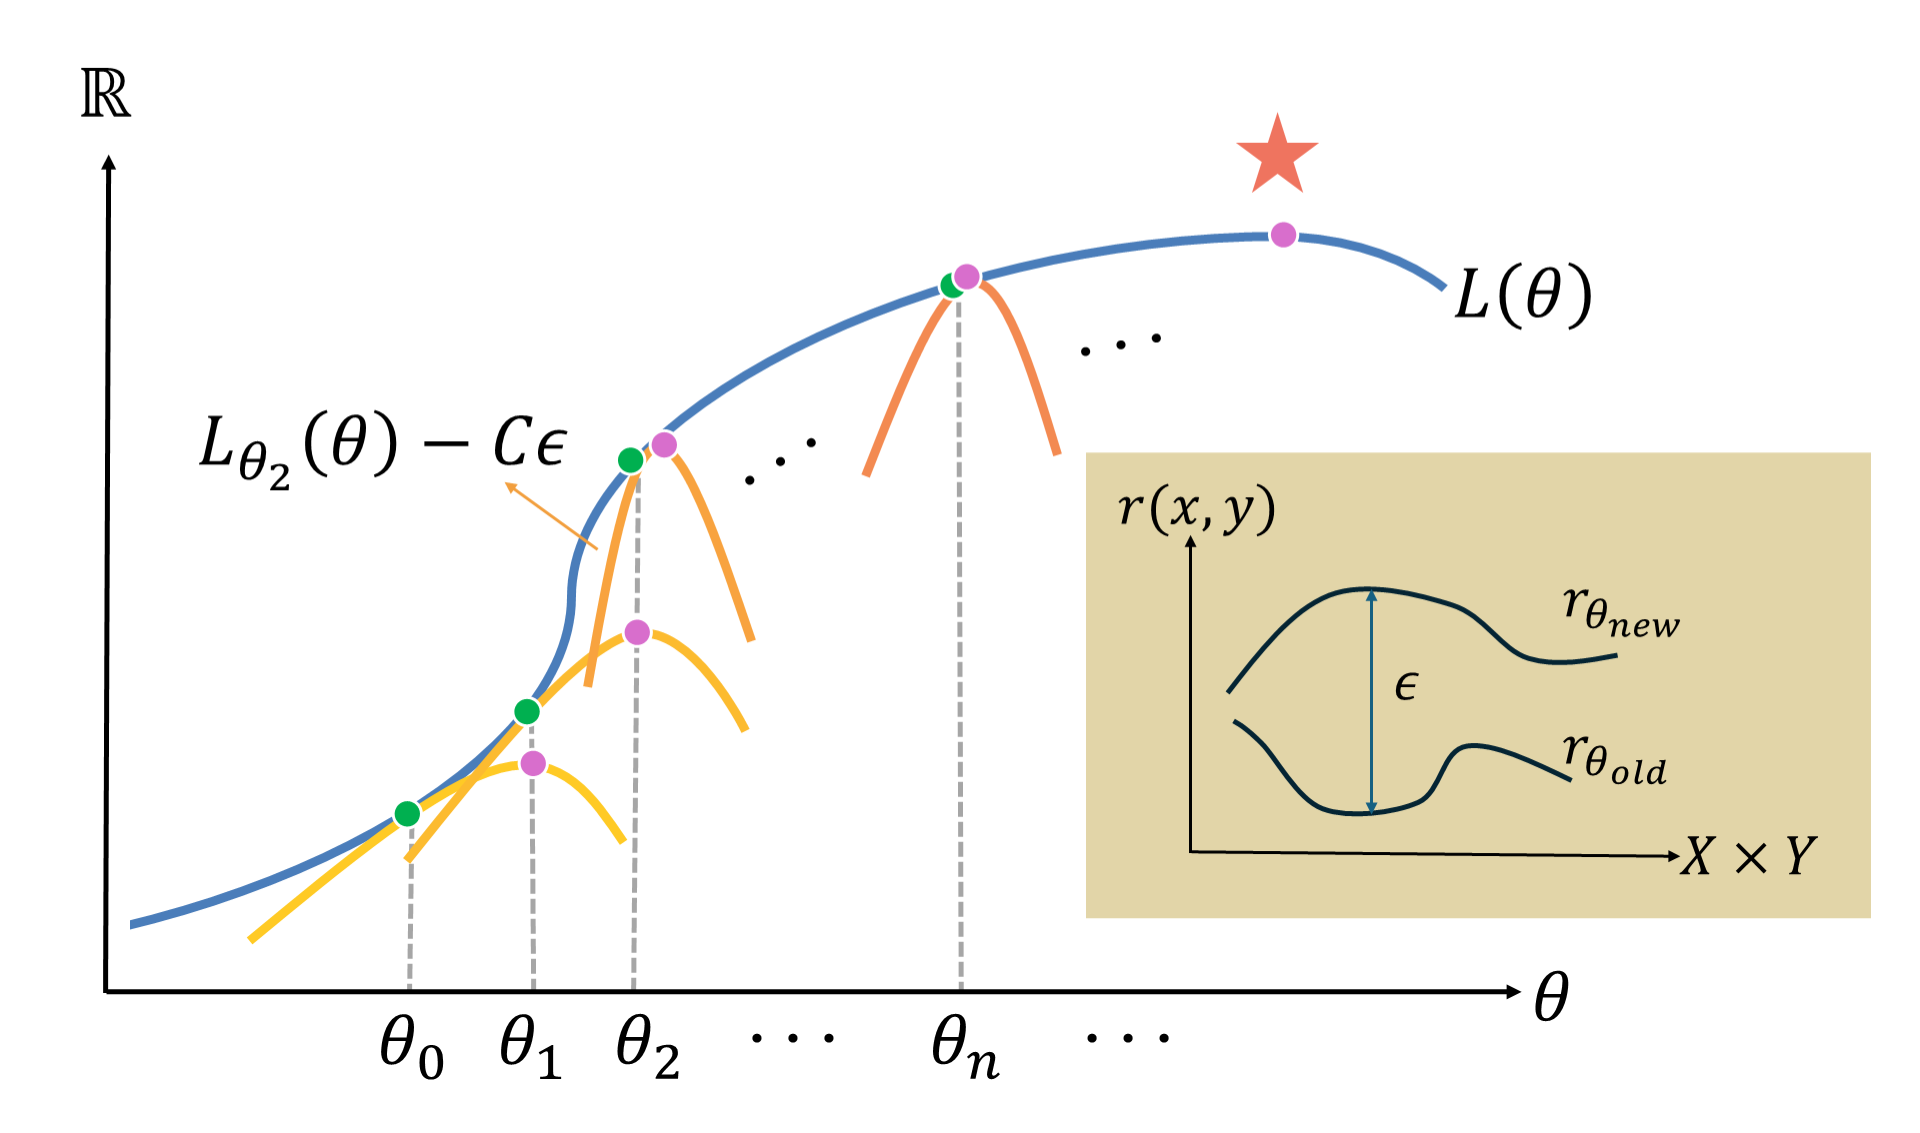
\includegraphics[width=0.95\textwidth]{figures/648.PNG}
    \caption{局部替代目标的下界与迭代优化示意}
    \label{fig:lower_bound_intuition}
\end{figure}

图~\ref{fig:lower_bound_intuition}给出了上述理论结果的直观解释。蓝色曲线表示原始目标 $L(\theta)$，橙色曲线表示以不同旧参数 $\theta_i$ 为展开点构造的局部替代下界。绿色点表示当前展开点，替代目标在该点与原始目标具有相同的一阶信息；紫色点表示沿替代目标更新后的候选参数。每一轮替代目标只在局部可信，若奖励函数更新过大，橙色下界与蓝色原始目标之间的偏差会增大，替代目标上的改进难以稳定对应到原始目标。右侧小图表示新旧奖励函数在样本空间 $\mathcal{X}\times\mathcal{Y}$ 上的逐点差异，$\epsilon$ 是这一差异的最大值。控制 $\epsilon$ 的作用是限制每一轮局部下界的失真程度，让多轮交替优化沿原始目标上升方向稳定推进。

据此，本文方法可以概括为围绕上述示意关系展开的交替过程。第 $k$ 轮开始时，先由当前奖励参数得到对应策略快照 $\pi_{\mathrm{old}}$；接着固定该策略快照，用专家响应与旧策略响应的奖励差异构造替代目标 $L_{\mathrm{old}}(\theta)-C\epsilon$，奖励更新时同时限制 $r_\theta$ 相对于 $r_{\theta_{\mathrm{old}}}$ 的变化幅度，避免替代目标过度偏离原始目标；将更新后的奖励参数作为下一轮的旧参数，继续优化策略。上述分析中，3.3节说明代理目标在展开点处具有相同的一阶方向，3.4节说明离开展开点后的代理误差可由奖励变化幅度控制，二者共同支持“受约束奖励更新”的方法原则。

\section{自适应约束调节机制}

\subsection{引入近似约束的必要性}

式~\eqref{eq:lower_bound}表明，替代目标与原始目标之间的偏差由误差项 $C\epsilon$ 控制。在实际训练中不能只最大化 $L_{\mathrm{old}}(\theta)$，还需限制相邻两轮奖励函数的变化幅度。然而，理论形式中的 $C$ 与 $\epsilon$ 都难以直接使用：$C$ 依赖完整响应空间大小 $|\mathcal{Y}|$，$\epsilon$ 需要在所有提示-响应对上取最大值。对于大语言模型，这两个量都无法直接计算。

为此，本文将理论约束转化为可计算的近似形式：用批次级统计量近似 $\epsilon$，用可调系数近似 $C$。这一步是从理论推导走向大模型训练算法的关键转换：PIRO并不要求枚举完整响应空间，而是在当前训练分布上观测奖励函数的跨轮变化，并据此调节奖励更新强度。

\subsection{\texorpdfstring{$\epsilon$}{epsilon} 的近似}

为近似理论中的最大逐点变化 $\epsilon$，本文使用相邻两轮奖励模型在同一批次样本上的均方根差。给定批次 $\mathcal{B}=\{(x^{(i)},y^{(i)})\}_{i=1}^{B}$，定义
\begin{equation}
    \text{RMSD}_k = \sqrt{\frac{1}{B}\sum_{i=1}^{B}\left(r_{\theta_k}(x^{(i)}, y^{(i)}) - r_{\theta_{k-1}}(x^{(i)}, y^{(i)})\right)^2}
    \label{eq:rmsd}
\end{equation}
其中 $\theta_k$ 和 $\theta_{k-1}$ 分别为第 $k$ 轮与第 $k-1$ 轮的奖励参数。RMSD不是全空间最大值 $\epsilon$ 的严格上界，而是训练批次上的可计算代理量，用于反映当前训练分布上的奖励变化强度。

\subsection{\texorpdfstring{$C$}{C} 的自适应近似}

理论常数 $C=3R|\mathcal{Y}|/\beta$ 无法在完整响应空间上直接计算。为在实现中保留 $C\epsilon$ 的约束作用，本文用可调系数 $\eta_k$ 近似 $C$，并根据RMSD反馈自适应更新 $\eta_k$。设 $\tau>0$ 为目标RMSD阈值，$\gamma\in(0,1)$ 为下阈值系数，$\delta>1$ 为上阈值系数，$\alpha\in(0,1)$ 为衰减因子，$\alpha'>1$ 为增长因子，调节规则为：

\begin{equation}
    \eta_{k+1} = \begin{cases}
        \alpha' \cdot \eta_k & \text{若 } \text{RMSD}_k > \delta\tau \\
        \alpha \cdot \eta_k & \text{若 } \text{RMSD}_k < \gamma\tau \\
        \eta_k & \text{其他}
    \end{cases}
    \label{eq:adaptive_eta}
\end{equation}
当RMSD大于上阈值 $\delta\tau$ 时，增大 $\eta_k$ 以加强对奖励变化的惩罚；当RMSD小于下阈值 $\gamma\tau$ 时，减小 $\eta_k$ 以放松约束。理论误差项 $C\epsilon$ 在实现中被近似为 $\eta_k\cdot\text{RMSD}_k$。

\section{完整训练流程}

\subsection{算法总体设计}

基于上述理论框架，本文提出近端逆奖励优化方法（Proximal Inverse Reward Optimization, PIRO）。其中，“奖励反演”表示从专家响应中学习可用于策略优化的奖励函数，“近端”表示每轮奖励更新受到相邻轮次奖励变化幅度的约束。PIRO采用奖励与策略交替优化的迭代训练范式，总体流程如算法~\ref{alg:piro}所示。

\begin{algorithm}[H]
    \caption{近端逆奖励优化算法（PIRO）}
    \label{alg:piro}
    \small
    \begin{algorithmic}[1]
        \Require 专家数据集 $\mathcal{D}_E$，提示数据集 $\mathcal{D}$，参考策略 $\pi_{\mathrm{ref}}$，
                 初始奖励参数 $\theta_0$，初始策略参数 $\phi_0$，
                 迭代轮数 $K$，每轮内层步数 $T_\pi$，每轮外层步数 $T_r$，
                 初始奖励学习率 $\lambda_0^r$，策略学习率 $\lambda^\pi$，初始约束系数 $\eta_0$，
                 RMSD目标阈值 $\tau$，下阈值系数 $\gamma$，上阈值系数 $\delta$，衰减因子 $\alpha$，增长因子 $\alpha'$
        \Ensure 对齐后的策略参数 $\phi$
        \State $\theta \gets \theta_0,\ \phi \gets \phi_0,\ \lambda^r \gets \lambda_0^r,\ \eta \gets \eta_0$
        \For{$k = 1, 2, \ldots, K$}
            \State \textbf{// 内层：策略优化}
            \For{$t = 1, 2, \ldots, T_\pi$}
                \State 从 $\mathcal{D}$ 采样批次提示 $\{x^{(i)}\}$，用当前策略 $\pi_{\phi}$ 采样响应 $\{y^{(i)}\}$
                \State 计算策略优化目标：$\mathcal{J}_\pi = \mathbb{E}\left[r_\theta(x,y) - \beta\log\frac{\pi_\phi(y|x)}{\pi_{\mathrm{ref}}(y|x)}\right]$
                \State 执行梯度上升：$\phi \gets \phi + \lambda^\pi \nabla_\phi \mathcal{J}_\pi$
            \EndFor
            \State \textbf{// 外层：奖励优化（含自适应约束）}
            \State 固定当前奖励参数与策略快照：$\theta_{\mathrm{old}} \gets \theta,\ \pi_{\mathrm{old}}\gets\pi_\phi$
            \For{$t = 1, 2, \ldots, T_r$}
                \State 从 $\mathcal{D}_E$ 采样专家响应批次 $\{(x^{(i)}, y_E^{(i)})\}$
                \State 从 $\mathcal{D}$ 采样提示，并用固定策略 $\pi_{\mathrm{old}}$ 采样响应批次 $\{(x^{(j)}, y_{\mathrm{old}}^{(j)})\}$
                \State 计算带批次RMSD惩罚的奖励目标 $L_{\mathrm{old}}(\theta)-\eta\cdot\text{RMSD}$
                \State $g_\theta \gets \nabla_\theta\left(\mathbb{E}[r_\theta(x,y_E)]-\mathbb{E}[r_\theta(x,y_{\mathrm{old}})]-\eta\cdot\text{RMSD}\right)$
                \State 执行梯度上升：$\theta \gets \theta + \lambda^r g_\theta$
            \EndFor
            \State \textbf{// 自适应约束系数调节}
            \State 在本轮奖励优化使用的样本批次上计算 $\text{RMSD}_k$（见式~\eqref{eq:rmsd}）
            \If{$\text{RMSD}_k > \delta\tau$}
                \State $\eta \gets \alpha' \cdot \eta$
            \ElsIf{$\text{RMSD}_k < \gamma\tau$}
                \State $\eta \gets \alpha \cdot \eta$
            \EndIf
        \EndFor
        \State \Return $\phi$
    \end{algorithmic}
\end{algorithm}

\subsection{算法流程说明}

算法~\ref{alg:piro}的训练流程由三个模块交替执行构成。

\textbf{内层策略优化}：固定当前奖励参数 $\theta$，以 $T_\pi$ 步梯度上升更新策略参数 $\phi$，让策略趋向当前奖励函数下的近似最优解。优化目标为期望奖励与KL惩罚的加权和，KL惩罚在词元级别计算，即 $\log(\pi_\phi(y|x)/\pi_{\mathrm{ref}}(y|x)) = \sum_t \log(\pi_\phi(a_t|s_t)/\pi_{\mathrm{ref}}(a_t|s_t))$。

\textbf{外层奖励优化}：固定当前策略为 $\pi_{\mathrm{old}}$，以 $T_r$ 步梯度上升更新奖励参数 $\theta$，最大化带批次RMSD惩罚的替代目标 $L_{\mathrm{old}}(\theta)-\eta\cdot\text{RMSD}$。本步固定 $\pi_{\mathrm{old}}$，KL项对 $\theta$ 不产生梯度，实现时用专家样本奖励减去旧策略样本奖励，并加入RMSD惩罚项来估计奖励更新方向。

\textbf{自适应约束系数调节}：每轮奖励优化完成后，计算本轮奖励函数相对于上轮的RMSD，依据式~\eqref{eq:adaptive_eta}调节下一轮的约束系数。当RMSD超过 $\delta\tau$ 时增大 $\eta$，当RMSD低于 $\gamma\tau$ 时减小 $\eta$。

\section{本章小结}

本章围绕受约束逆强化学习的大模型对齐方法展开，主要内容包括：（1）将对齐问题写成专家响应似然最大化的双层目标，外层学习奖励参数，内层求解KL正则最优策略；（2）推导内层问题的Boltzmann闭式策略，说明奖励通过指数加权影响参考策略；（3）构造固定旧策略的替代目标，并说明其与原始目标在展开点处一阶一致；（4）给出改进下界，说明原始目标不低于替代目标减去误差项 $C\epsilon$，奖励更新幅度需要受控；（5）在实际实现中用批次RMSD监控奖励变化，并据此自适应调整约束系数。至此，基于逆强化学习的偏好奖励反演被转化为PIRO的可执行训练流程：奖励函数可以随策略分布更新，但其跨轮变化必须受到近端约束。第四章将通过实验检验该约束机制对对齐效果和训练稳定性的影响。
